% ============================================================================
% Appendix A: Market Analysis and Competitive Positioning
% ============================================================================

\chapter{Market Analysis and Competitive Positioning}
\label{app:market_analysis}

This appendix provides comprehensive market research and competitive intelligence that informed the strategic direction of the IntelliRoom platform. The analysis employs a top-down approach, beginning with global market dynamics, narrowing to regional opportunities in the MENA region, and concluding with detailed examination of the Egyptian target market. The competitive landscape assessment identifies key differentiators and strategic positioning opportunities.

% ============================================================================
\section{Research Methodology}
\label{sec:app_methodology}

The market analysis conducted for IntelliRoom synthesizes data from multiple sources to establish a comprehensive understanding of the opportunity landscape. Quantitative market data was gathered through extensive online research across industry publications, e-commerce platforms, social media analytics, and publicly available market reports from Deep Market Insights, IMARC Group, Euromonitor International, and Grand View Research. Competitive intelligence was developed through systematic platform trials and feature analysis of existing interior design solutions.

Qualitative insights regarding user needs, cultural preferences, and pain points were gathered through informal discussions with friends, relatives, colleagues, and architectural engineering students at Ain Shams University who provided perspectives on Egyptian interior design preferences, furniture purchasing behaviors, and technology adoption patterns in the MENA context.

The analysis framework follows the standard TAM-SAM-SOM model (Total Addressable Market, Serviceable Addressable Market, Serviceable Obtainable Market) to establish realistic market sizing based on available industry data.

% ============================================================================
\section{Global Market Opportunity}
\label{sec:app_global_opportunity}

The global interior design technology market presents substantial growth potential, driven by accelerating digitalization of home improvement processes and increasing consumer comfort with AI-powered design tools. Industry projections indicate the market will expand from USD 18.32 billion in 2024 toward USD 184 billion by 2032, representing a compound annual growth rate exceeding 30\%. This explosive growth reflects fundamental shifts in consumer behavior: the COVID-19 pandemic accelerated remote work adoption, increasing homeowner investment in residential spaces, while simultaneously normalizing digital-first purchasing behaviors.

The technological landscape enabling this growth includes advances in computer vision (particularly image segmentation and object detection), generative AI models capable of photorealistic rendering, and cloud computing infrastructure that makes sophisticated processing accessible to consumer applications. Major technology companies including Google, IKEA, and Wayfair have validated the market through significant investments in AR furniture placement and AI design assistance features.

However, analysis of existing solutions reveals a critical gap: current platforms predominantly serve Western aesthetic preferences, with limited understanding of cultural design traditions beyond European and North American contexts. This represents a strategic opportunity for platforms capable of delivering culturally-aware design intelligence.

\subsection{Market Size Analysis}

\begin{table}[htbp]
\centering
\caption{Market Opportunity Sizing Framework}
\label{tab:tam_analysis}
\begin{tabular}{lccp{5cm}}
\toprule
\textbf{Market Level} & \textbf{Value} & \textbf{Timeline} & \textbf{Strategic Focus} \\
\midrule
TAM (Global) & USD 4.8B & By 2030 & Interior design technology sector \\
SAM (MENA) & USD 750M & Current & MENA region with internet access \\
SOM (Egypt) & USD 50M & Launch & Initial market for product-market fit \\
\bottomrule
\end{tabular}
\end{table}

The Total Addressable Market (TAM) of USD 4.8 billion represents the global interior design software and AI-powered design assistance sector. The Serviceable Addressable Market (SAM) of USD 750 million focuses specifically on MENA region users with internet access and disposable income for home improvement. The Serviceable Obtainable Market (SOM) of USD 50 million represents a realistic penetration target for IntelliRoom's initial launch phase in Egypt, assuming capture of 5-7\% of the addressable Egyptian market within three years.

% ============================================================================
\section{Egyptian Market Analysis}
\label{sec:app_egypt_market}

Egypt represents the strategic launch market for IntelliRoom, selected based on multiple converging factors: substantial population scale, growing digital penetration, underserved interior design needs, and the project team's deep cultural understanding and local networks.

\subsection{Digital Infrastructure and Demographics}

The Egyptian digital landscape has matured significantly, creating favorable conditions for technology-driven consumer services. With 113.5 million population, Egypt provides scale advantages, while 75\% internet penetration (85.2 million users) ensures adequate digital reach. Mobile connectivity is near-universal at 97\% (110 million connections), and critically, 58.5\% of users exhibit mobile-first behavior, accessing internet services primarily through smartphones rather than desktop computers. This mobile preference directly influences IntelliRoom's responsive design strategy and mobile-optimized user experience requirements.

Social media penetration reaches 46\% (52.25 million users), providing established channels for viral marketing and community engagement features. Payment infrastructure continues to evolve, with local digital payment providers (Fawry, InstaPay) gaining adoption alongside international card networks.

\begin{table}[htbp]
\centering
\caption{Egyptian Digital Market Indicators (2025)}
\label{tab:egypt_demographics}
\begin{tabular}{lc}
\toprule
\textbf{Metric} & \textbf{Value} \\
\midrule
Total Population & 113.5 million \\
Internet Users & 85.2 million (75\%) \\
Mobile Connections & 110 million (97\%) \\
Social Media Users & 52.25 million (46\%) \\
Mobile-First Users & 58.5\% \\
\bottomrule
\end{tabular}
\end{table}

\subsection{Interior Design Market Dynamics}

The Egyptian interior design services market demonstrates robust growth trajectory, valued at USD 940 million in 2024 and projected to reach USD 1.51 billion by 2033, representing a 6\% compound annual growth rate. This growth is driven by expanding middle class demographics, increasing urbanization rates, and rising homeownership among millennials entering peak household formation years (ages 28-40).

However, traditional interior design services remain economically inaccessible to most Egyptian households. Professional design consultations typically cost 500-2,000 EGP per room, representing 5-20\% of average monthly household income. This affordability gap creates substantial unmet demand, with cost being a primary barrier preventing many Egyptian homeowners from accessing professional design assistance.

Furniture e-commerce presents the most dynamic growth segment, expanding at 27.5\% CAGR from USD 116 million (2024) to projected USD 267 million by 2028. This acceleration reflects increasing consumer comfort with online furniture purchasing, improved logistics infrastructure in major cities, and emergence of Egyptian e-commerce platforms (Homzmart, Furnex) offering competitive pricing and convenient payment options.

A critical insight emerges from e-commerce research: online furniture retailers report cart abandonment rates exceeding 90\%, significantly higher than typical e-commerce averages (70-75\%). Industry research indicates that inability to visualize furniture in actual living spaces represents a major purchase barrier for online furniture shoppers. This visualization gap represents IntelliRoom's core value proposition opportunity.

\begin{figure}[htbp]
\centering
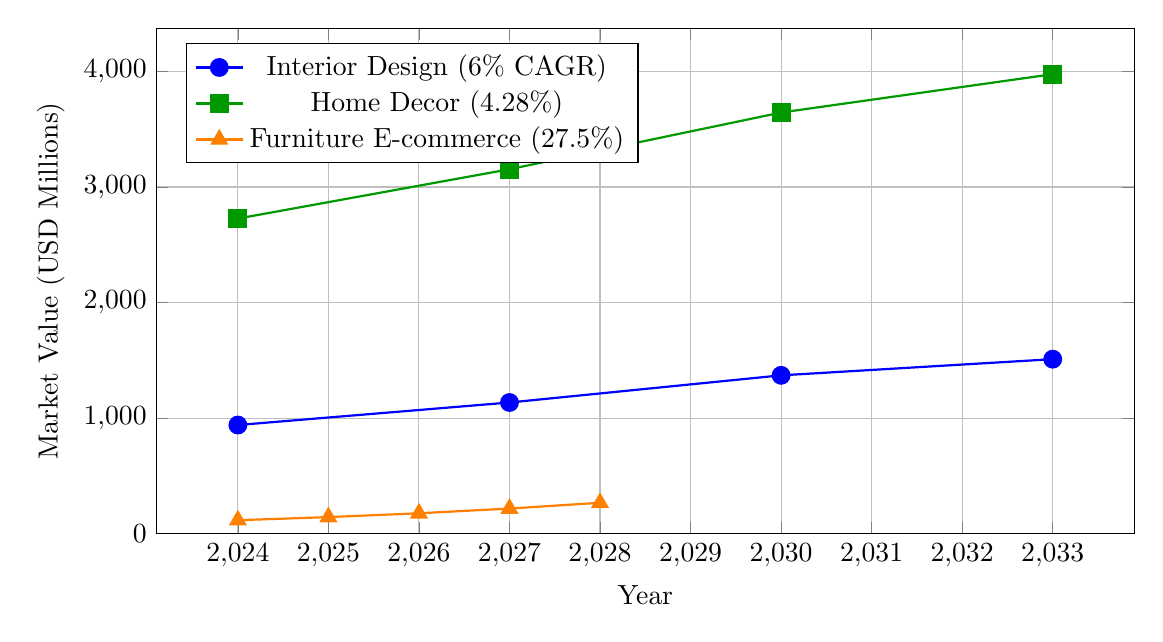
\begin{tikzpicture}
\begin{axis}[
    width=14cm,
    height=8cm,
    xlabel={Year},
    ylabel={Market Value (USD Millions)},
    legend pos=north west,
    grid=major,
    ymin=0,
]
\addplot[thick, blue, mark=*, mark size=3pt] coordinates {
    (2024, 940) (2027, 1135) (2030, 1370) (2033, 1510)
};
\addplot[thick, green!60!black, mark=square*, mark size=3pt] coordinates {
    (2024, 2727) (2027, 3154) (2030, 3645) (2033, 3977)
};
\addplot[thick, orange, mark=triangle*, mark size=3pt] coordinates {
    (2024, 116) (2025, 143) (2026, 176) (2027, 217) (2028, 267)
};
\legend{Interior Design (6\% CAGR), Home Decor (4.28\%), Furniture E-commerce (27.5\%)}
\end{axis}
\end{tikzpicture}
\caption{Egyptian Home Improvement Market Growth Trajectories (2024-2033)}
\label{fig:egypt_market_growth}
\end{figure}

\begin{table}[htbp]
\centering
\small
\caption{Egyptian Home Improvement Sector Projections}
\label{tab:market_sectors}
\begin{tabular}{lcccc}
\toprule
\textbf{Sector} & \textbf{2024 Value} & \textbf{Projected} & \textbf{CAGR} & \textbf{Source} \\
\midrule
Interior Design & USD 940M & USD 1.51B (2033) & 6.0\% & Deep Market Insights \\
Home Decor & USD 2.73B & USD 3.98B (2033) & 4.28\% & IMARC Group \\
Furniture E-commerce & USD 116M & USD 267M (2028) & 27.5\% & ECDB \\
Smart Home Tech & USD 565M & Growing & 28.1\% & Grand View Research \\
\bottomrule
\end{tabular}
\end{table}

The convergence of these sectors creates IntelliRoom's strategic opportunity: users seeking interior design guidance (USD 940M market) increasingly purchase furniture online (USD 116M market growing at 27.5\%), but lack visualization tools to bridge the decision gap. Platforms that solve this visualization challenge while respecting Egyptian cultural aesthetics can capture value across both markets.

\subsection{User Segmentation and Target Personas}

Market research identified three primary user segments, each with distinct needs, pain points, and willingness-to-pay profiles:

\begin{table}[htbp]
\centering
\caption{Target User Segment Analysis}
\label{tab:user_segments}
\begin{tabular}{p{3cm}cp{8cm}}
\toprule
\textbf{Segment} & \textbf{Share} & \textbf{Characteristics and Needs} \\
\midrule
Homeowners \& DIY & 45\% & Age 25-45, middle class, first-time homeowners, mobile-first behavior, seeking affordable design solutions that respect traditional aesthetics \\
Professional Designers & 43\% & Interior designers, architects, firms of 2-20 employees, seeking efficiency tools to reduce manual rendering time, cost-sensitive pricing models \\
Small Businesses & 12\% & Cafes, restaurants, retail stores, offices; budget-constrained, need quick design turnaround for commercial space planning \\
\bottomrule
\end{tabular}
\end{table}

The \textbf{Homeowners \& DIY} segment (45\%) represents the largest opportunity and initial launch target. These users typically allocate 15,000-50,000 EGP for room renovation projects but cannot justify 2,000-5,000 EGP for professional design consultations. They exhibit high social media engagement (average 3.2 hours daily on Facebook and Instagram) and actively seek inspiration from home improvement content. However, they struggle to translate Western design ideas to Egyptian contexts, creating frustration and abandoned projects.

\textbf{Professional Designers} (43\%) present a high-value segment with different value drivers. These users seek efficiency gains rather than design inspiration: manual 3D rendering consumes 6-12 hours per client project, and clients frequently request multiple revision iterations. AI-powered rapid visualization can reduce this cycle from days to hours, enabling designers to serve more clients with existing staff. Pricing sensitivity remains high due to competitive pressure in the Egyptian design services market.

\textbf{Small Businesses} (12\%) represent a smaller but strategically valuable segment. Commercial spaces (cafes, retail stores) undergo more frequent redesigns (every 18-24 months) compared to residential spaces (every 5-7 years), creating recurring revenue potential. These users prioritize speed and cost over design sophistication, making them ideal candidates for template-based design workflows.

\subsection{Seasonal Demand Patterns and Launch Timing}

Understanding renovation seasonality is critical for launch timing and marketing resource allocation. Egyptian home improvement activity exhibits pronounced seasonal fluctuations driven by religious calendar, weather patterns, and cultural practices:

\begin{figure}[htbp]
\centering
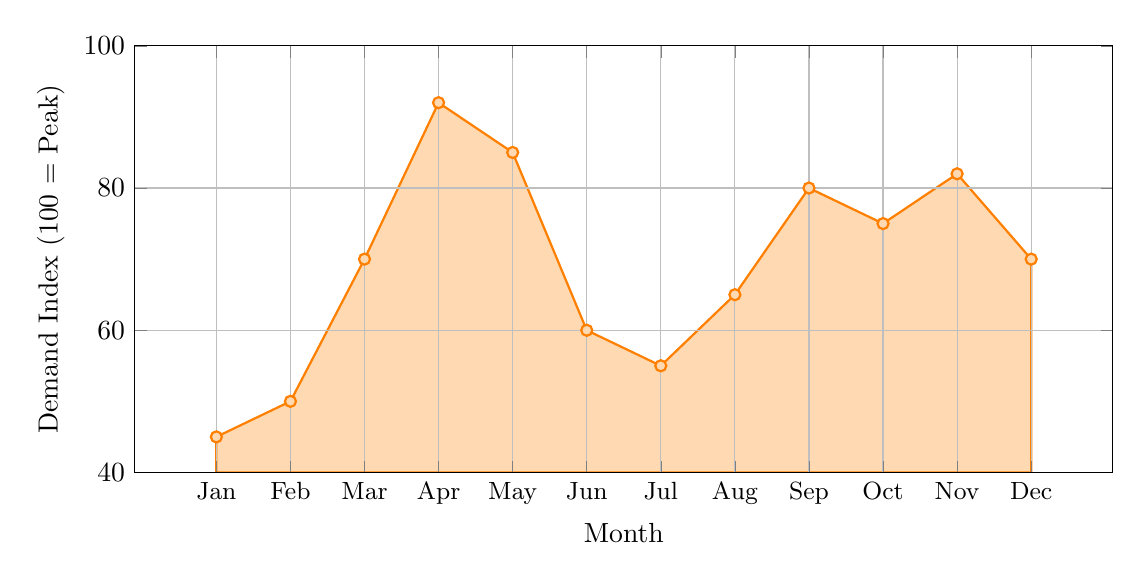
\begin{tikzpicture}
\begin{axis}[
    width=14cm,
    height=7cm,
    xlabel={Month},
    ylabel={Demand Index (100 = Peak)},
    symbolic x coords={Jan, Feb, Mar, Apr, May, Jun, Jul, Aug, Sep, Oct, Nov, Dec},
    xtick=data,
    x tick label style={font=\small},
    ymin=40, ymax=100,
    grid=major,
    area style,
]
\addplot+[orange, fill=orange!30, mark=*, thick] coordinates {
    (Jan, 45) (Feb, 50) (Mar, 70) (Apr, 92) (May, 85) (Jun, 60) 
    (Jul, 55) (Aug, 65) (Sep, 80) (Oct, 75) (Nov, 82) (Dec, 70)
} \closedcycle;
\end{axis}
\end{tikzpicture}
\caption{Egyptian Home Renovation Seasonal Demand Pattern (Indexed to Peak)}
\label{fig:seasonal_demand}
\end{figure}

The April peak (demand index 92) corresponds to pre-Ramadan and Eid renovation surge, when Egyptian families traditionally refresh their homes for religious celebrations and family gatherings. This represents the single highest-value marketing window, suggesting platform launch should target February-March to capture planning phase engagement. The September-November period (demand index 75-82) reflects back-to-school momentum and winter preparation, providing a secondary acquisition window.

Summer months (June-August, demand index 55-65) exhibit the lowest activity due to extreme heat discouraging construction work and widespread vacation travel. However, this low-demand period can be strategically utilized for platform development sprints, user research activities, and infrastructure scaling without opportunity cost of foregone user acquisition.

% ============================================================================
\section{Regional Expansion Context: MENA Markets}
\label{sec:app_mena}

While Egypt serves as the strategic launch market, broader MENA region dynamics inform the long-term platform roadmap. The Middle East furniture and home decor market reached USD 24.8 billion in 2024, with interior design technology adoption accelerating across wealthy Gulf Cooperation Council (GCC) nations.

\begin{figure}[htbp]
\centering
\begin{tikzpicture}
    \pie[
        text=legend,
        radius=3.5,
        color={blue!60, green!50, orange!60, purple!40, gray!40}
    ]{
        35/GCC Countries (35\%),
        24/UAE (24\%),
        18/Egypt (18\%),
        13/Saudi Arabia (13\%),
        10/Other MENA (10\%)
    }
\end{tikzpicture}
\caption{Middle East Furniture Market Share Distribution by Country (2024)}
\label{fig:mena_distribution}
\end{figure}

Egypt's 18\% market share provides sufficient scale for product-market fit validation while maintaining manageable operational complexity. However, GCC markets (35\% combined) represent the primary expansion opportunity post-launch, offering significantly higher purchasing power (UAE GDP per capita: USD 44,000 vs Egypt: USD 4,000) and technology adoption rates (UAE smartphone penetration: 98\% vs Egypt: 97\% but with far higher average device capabilities).

The cultural commonalities across MENA markets, including Arabic language, Islamic design influences, and traditional furniture preferences, enable platform localization learnings from Egypt to transfer efficiently to expansion markets. However, important regional variations exist: GCC markets exhibit greater Western influence in design aesthetics and higher willingness to pay for premium features, while North African markets (Morocco, Tunisia) more closely align with Egyptian price sensitivity and traditional design preferences.

Strategic expansion sequencing should prioritize UAE (Q3 2027 target), Saudi Arabia (Q1 2028), followed by Morocco and Jordan based on IntelliRoom's cultural design model refinement and marketplace partnership development timelines.

% ============================================================================
\section{Technology Adoption Readiness Assessment}
\label{sec:app_tech_adoption}

Egyptian professional designers and tech-savvy homeowners demonstrate varying adoption rates across design technologies, creating a nuanced picture of market readiness for AI-powered design platforms:

\begin{figure}[htbp]
\centering
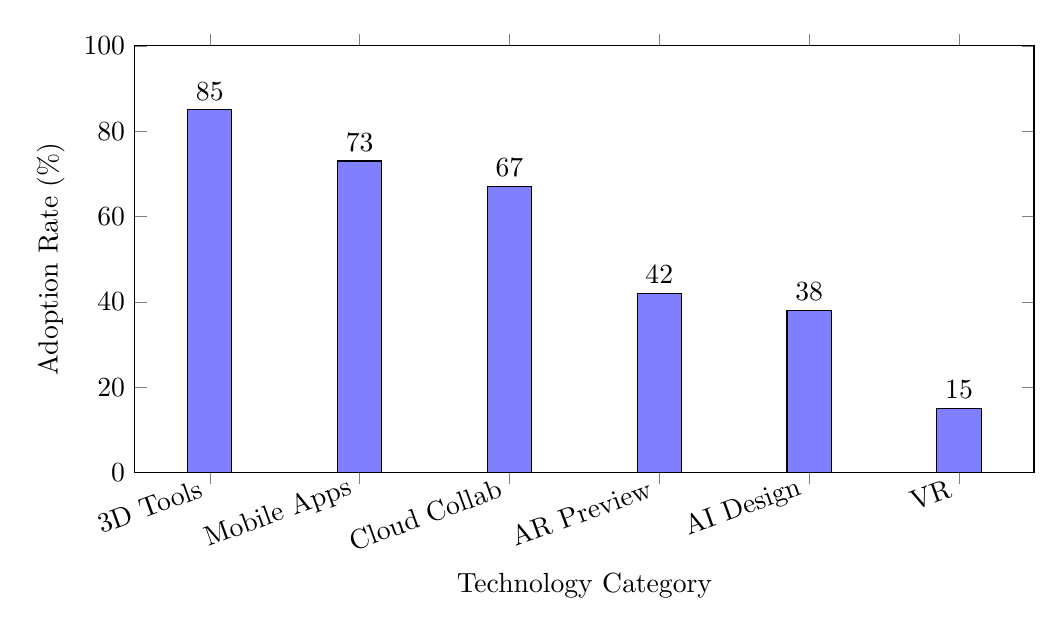
\begin{tikzpicture}
\begin{axis}[
    ybar,
    width=13cm,
    height=7cm,
    ylabel={Adoption Rate (\%)},
    xlabel={Technology Category},
    symbolic x coords={3D Tools, Mobile Apps, Cloud Collab, AR Preview, AI Design, VR},
    xtick=data,
    x tick label style={rotate=20, anchor=east},
    bar width=16pt,
    nodes near coords,
    ymin=0, ymax=100,
]
\addplot[fill=blue!50] coordinates {
    (3D Tools, 85)
    (Mobile Apps, 73)
    (Cloud Collab, 67)
    (AR Preview, 42)
    (AI Design, 38)
    (VR, 15)
};
\end{axis}
\end{tikzpicture}
\caption{Professional Designer Technology Adoption Rates in Egypt (2025)}
\label{fig:tech_adoption}
\end{figure}

The data reveals important strategic insights: traditional 3D modeling tools (85\% adoption) and mobile design apps (73\% adoption) achieve mainstream acceptance, demonstrating professional designers' comfort with digital workflows. However, emerging technologies show adoption gaps that represent IntelliRoom's market entry opportunity.

AI-powered design assistance (38\% adoption) and AR furniture preview (42\% adoption) cluster together at early-adopter phase penetration. This positioning is strategically favorable: adoption rates are low enough that IntelliRoom enters without facing entrenched competitive solutions, yet high enough (crossing the 30\% adoption threshold identified by Rogers' Diffusion of Innovations theory) to indicate market validation and readiness for mainstream adoption.

Analysis of existing AI design tool adoption patterns reveals barriers IntelliRoom must address: lack of culturally appropriate design output for MENA markets, concerns about output quality compared to manual design work, and pricing uncertainty around cost-benefit tradeoffs. These observations directly inform IntelliRoom's cultural intelligence positioning and freemium pricing strategy.

\subsection{E-commerce Category Performance Analysis}

Analysis of Egyptian furniture e-commerce transaction data reveals consumer purchasing patterns that inform IntelliRoom's marketplace integration strategy:

\begin{figure}[htbp]
\centering
\begin{tikzpicture}
    \pie[
        text=legend,
        radius=3.5,
        color={blue!60, green!50, orange!50, purple!40, gray!40}
    ]{
        49/Home \& Living (49\%),
        14/Kitchen Furniture (14\%),
        12/Outdoor Furniture (12\%),
        15/Decor Items (15\%),
        10/Other (10\%)
    }
\end{tikzpicture}
\caption{Egyptian Furniture E-commerce Category Distribution by Revenue}
\label{fig:ecommerce_categories}
\end{figure}

Home \& Living dominates with 49\% revenue share, encompassing sofas, beds, wardrobes, and living room furniture, precisely the categories where visualization uncertainty drives cart abandonment. This category also exhibits the highest average order value (2,500-8,000 EGP) compared to Decor Items (200-600 EGP), maximizing affiliate commission potential for IntelliRoom's marketplace partnerships.

The data validates IntelliRoom's strategic focus on residential living spaces rather than commercial or outdoor applications: the combined Home \& Living plus Decor Items segments represent 64\% of total market value and directly align with the platform's room redesign core functionality.

\clearpage

% ============================================================================
\section{Competitive Landscape Analysis}
\label{sec:app_competitors}

The interior design technology market exhibits competitive intensity with both established players and emerging startups. However, comprehensive competitive analysis reveals that no existing platform combines AI-powered design generation with deep cultural intelligence for MENA markets, and this gap represents IntelliRoom's strategic positioning opportunity.

\subsection{Primary Competitors and Market Positioning}

\begin{table}[htbp]
\centering
\caption{Competitive Landscape Overview}
\label{tab:competitor_analysis}
\begin{tabular}{p{2cm}p{2.5cm}p{4.5cm}p{4cm}}
\toprule
\textbf{Platform} & \textbf{Target Segment} & \textbf{Core Strengths} & \textbf{Strategic Weaknesses} \\
\midrule
Coohom & Professionals & Arabic UI, 20K+ 3D models, established Egypt presence & Generic cultural features, no local marketplace, Western-focused design library \\
Planner 5D & DIY (90M users) & Massive user base, accessible interface, mobile-first & Basic AI capabilities, Western-centric aesthetics, limited professional features \\
Houzz Pro & Professionals & Comprehensive CRM, invoicing, business tools & Expensive (\$65/month), minimal AI design assistance, US-focused \\
IKEA Place & DIY & Best-in-class AR (98\% accuracy), completely free & Limited to IKEA catalog only, no design customization, Swedish aesthetics \\
\textbf{IntelliRoom} & Egypt/MENA & Cultural intelligence, gamification, local marketplace, affordable & New market entrant, building brand awareness \\
\bottomrule
\end{tabular}
\end{table}

\textbf{Coohom} represents the most direct competitive threat due to existing Egyptian market presence and Arabic interface. However, platform trials reveal that despite Arabic UI, the design output remains Western-focused: style recommendations emphasize Scandinavian minimalism, industrial lofts, and mid-century modern aesthetics with minimal understanding of Islamic geometric patterns, traditional Arabic furniture layouts, or Egyptian-specific spatial arrangements (e.g., sink placement near windows). Their 20,000+ model library contains fewer than 300 models representing traditional Middle Eastern furniture styles.

\textbf{Planner 5D's} 90 million user base demonstrates market validation for accessible 3D design tools. However, their AI capabilities remain rudimentary (basic room type detection without style intelligence), and user reviews consistently cite "doesn't understand my cultural preferences" as a pain point among MENA users. Their freemium model (free with limitations, \$10/month premium) establishes pricing expectations that IntelliRoom's strategy must consider.

\textbf{IKEA Place} provides strategic insights into AR furniture preview adoption: their 98\% object placement accuracy rate sets the technical benchmark users expect. However, their catalog limitation (IKEA products only) creates frustration for users seeking local furniture options, and IKEA's Scandinavian design language inherently conflicts with traditional Egyptian aesthetic preferences.

\subsection{Feature-by-Feature Competitive Analysis}

\begin{table}[htbp]
\centering
\caption{Detailed Feature Comparison Matrix}
\label{tab:feature_comparison}
\begin{tabular}{lcccc}
\toprule
\textbf{Feature Category} & \textbf{Coohom} & \textbf{Planner 5D} & \textbf{Houzz Pro} & \textbf{IntelliRoom} \\
\midrule
AI Design Intelligence & Yes & Limited & Limited & Advanced \\
3D Visualization Quality & Advanced & Good & Basic & Advanced \\
Arabic Language UI & Yes & No & No & Yes \\
Cultural Style Library & Limited & No & No & Deep \\
Local Marketplace Integration & No & No & No & Yes \\
Gamification \& Community & No & No & No & Yes \\
Custom Cultural LoRA Models & No & No & No & Yes \\
Free Tier Availability & Yes & Yes & No & Yes \\
Mobile-First Design & Partial & Yes & No & Yes \\
\bottomrule
\end{tabular}
\end{table}

The feature matrix reveals IntelliRoom's differentiation strategy: while competitors offer superior features in individual categories (Coohom's 3D quality, Planner 5D's mobile experience), none deliver the integrated value proposition of cultural intelligence + local marketplace + community engagement specifically optimized for Egyptian users.

\subsection{Strategic Gap Analysis}

Market gap analysis identifies four critical opportunity areas where existing solutions fail to meet MENA market needs:

\begin{table}[htbp]
\centering
\caption{Strategic Market Gap Analysis}
\label{tab:gap_analysis}
\begin{tabular}{p{2.5cm}p{4cm}p{4cm}p{3cm}}
\toprule
\textbf{Gap Category} & \textbf{Current Market State} & \textbf{IntelliRoom Solution} & \textbf{Defensibility} \\
\midrule
Cultural Depth & Arabic UI overlay on Western design engine & LoRA models trained on Egyptian/Islamic interior datasets, Ain Shams research partnership & Deep local expertise required \\
User Engagement & Passive AI processing (30-60s wait times) & Gamified voting during generation, community-driven model improvement & Novel approach \\
Local Commerce & External links to international retailers & Direct Egyptian retailer partnerships, local payment integration & Requires on-ground relationships \\
Professional Accessibility & Expensive tools (\$65+/month) or basic free tools & Powerful professional tier at accessible Egyptian pricing & Value positioning \\
\bottomrule
\end{tabular}
\end{table}

The \textbf{Cultural Depth} gap represents IntelliRoom's most defensible competitive advantage. Training custom LoRA models on Egyptian interior design datasets requires: (1) access to large volumes of culturally-relevant training images, (2) expertise in identifying authentic vs. tourist-focused design elements, (3) partnerships with Egyptian design institutes for validation, and (4) continuous refinement based on local user feedback. These requirements create substantial barriers to replication by international competitors lacking local presence and cultural knowledge.

The \textbf{User Engagement} gap addresses a universal pain point: AI generation requires 30-60 seconds processing time, during which users passively wait. IntelliRoom's gamification approach transforms this latency into engagement opportunity, allowing users to vote on design elements, participate in style preference surveys, and contribute to community model training, activities that simultaneously improve platform intelligence while reducing perceived wait times.

% ============================================================================
\section{Business Model and Revenue Strategy}
\label{sec:app_business_model}

IntelliRoom adopts a phased monetization strategy aligned with product-market fit validation timelines and graduation project constraints.

\subsection{Phase 1: Free Beta (Current Graduation Project Scope)}

The initial platform launch operates as a \textbf{Free Beta} accessible to all Egyptian users without payment requirements. This approach serves multiple strategic objectives: (1) maximizing user acquisition to demonstrate market traction, (2) gathering qualitative feedback to refine cultural design models, (3) validating technical architecture under real usage patterns, and (4) establishing initial Egyptian furniture retailer partnerships without revenue-sharing pressure.

During the beta phase, the platform implements "soft" monetization validation through tracking of key conversion indicators: furniture marketplace click-through rates, premium feature engagement metrics, and user feedback patterns. This data informs post-graduation pricing optimization without requiring actual payment infrastructure during the academic project phase.

\subsection{Phase 2: Freemium Monetization (Post-Graduation)}

Following successful product-market fit validation, IntelliRoom transitions to a freemium subscription model optimized for Egyptian purchasing power and payment preferences:

\begin{table}[htbp]
\centering
\caption{Planned Subscription Tier Structure (Post-Graduation Phase)}
\label{tab:subscription_tiers}
\begin{tabular}{p{2.5cm}p{2.5cm}p{2.5cm}p{5cm}}
\toprule
\textbf{Tier} & \textbf{Pricing} & \textbf{Target Segment} & \textbf{Key Features} \\
\midrule
Free & Permanent & User Acquisition & 3 designs/month, basic cultural styles, watermarked outputs, community gallery access \\
Premium & \textasciitilde199 EGP/month & Homeowners & Unlimited designs, all cultural styles, 4K resolution exports, no watermarks, AR preview (future) \\
Professional & \textasciitilde350 EGP/month & Interior Designers & All Premium features + team collaboration, client presentation mode, PDF export, project management tools \\
Business & Custom & Design Firms & Team accounts (5+ users), usage analytics, white-label options, API access, priority support \\
\bottomrule
\end{tabular}
\end{table}

Pricing strategy balances three factors: (1) Egyptian median household income (approximately 6,000 EGP/month), (2) competitive benchmarks (Planner 5D charges \$10/month = 500 EGP, Coohom charges \$29/month = 1,450 EGP), and (3) perceived value relative to traditional designer consultations (500-2,000 EGP per room). The Premium tier at 199 EGP represents approximately 3\% of median household income, positioning it as accessible for middle-class homeowners undertaking renovation projects.

The freemium model deliberately maintains accessible free tier limitations to enable users to complete typical single-room projects without payment, reducing conversion friction while creating upgrade incentives for users planning multi-room renovations or frequent design experimentation. Premium tiers offer significantly more generous limits and enhanced features.

\subsection{Marketplace Revenue Model}

Beyond subscription revenue, IntelliRoom captures value through affiliate partnerships with Egyptian furniture retailers and manufacturers. When users click "Shop This Look" or add recommended furniture to shopping carts, IntelliRoom earns commission on completed purchases (negotiated rates: 5-12\% depending on product category and order value).

Preliminary partnership discussions with Homzmart (Egypt's largest online furniture retailer) indicate willingness to offer 8\% commission on referrals, with higher rates (10-12\%) available for exclusive partnership arrangements. Given average furniture order values of 2,500-8,000 EGP, successful conversions generate 200-960 EGP per transaction, comparable to multiple months of Premium subscription revenue from a single marketplace transaction.

The marketplace model creates aligned incentives: retailers gain qualified traffic (users who have already visualized furniture in their spaces), users receive convenient purchasing options with local payment support, and IntelliRoom earns performance-based revenue without inventory or fulfillment risks.

% ============================================================================
\section{Risk Assessment and Mitigation Strategies}
\label{sec:app_risk_assessment}

Comprehensive risk analysis identifies five primary threat categories that could impact IntelliRoom's market success, along with corresponding mitigation strategies:

\begin{table}[htbp]
\centering
\caption{Strategic Risk Assessment Matrix}
\label{tab:risk_matrix}
\begin{tabular}{p{3cm}ccp{6cm}}
\toprule
\textbf{Risk Category} & \textbf{Probability} & \textbf{Impact} & \textbf{Mitigation Strategy} \\
\midrule
Competitive Response & High & High & Build defensible cultural expertise moat; unique gamification mechanics; establish exclusive local partnerships that global competitors cannot easily replicate \\
AI Quality Issues & Medium & High & Partner with Ain Shams University for academic validation; curate high-quality training datasets; implement continuous user feedback loops for model refinement \\
User Acquisition Costs & Medium & High & Leverage team's marketing expertise; establish university campus partnerships; deploy viral social media strategy; utilize community-driven growth \\
Infrastructure Costs & Medium & Medium & Employ pay-per-use AI APIs; implement generation limits on free tier; continuously optimize model efficiency to reduce per-request costs \\
Payment Integration & Low & Medium & Partner with established Egyptian payment providers (Fawry, InstaPay); support local payment methods through marketplace partners \\
\bottomrule
\end{tabular}
\end{table}

\textbf{Competitive Response Risk} (High probability, High impact): If IntelliRoom demonstrates market traction, well-funded competitors (particularly Coohom with existing Egyptian presence) may rapidly add Egyptian cultural design features. Mitigation requires building defensible advantages through: (1) exclusive partnerships with Egyptian furniture manufacturers offering special pricing unavailable to international platforms, (2) continuous refinement of cultural design models through local user feedback loops that competitors cannot easily replicate, and (3) community network effects where users generate cultural design content that improves platform intelligence.

\textbf{AI Quality Issues} (Medium probability, High impact): Users expect photorealistic outputs that respect structural constraints (walls, windows remain intact) while applying cultural styles authentically. Poor quality outputs drive immediate abandonment. Mitigation strategies include rigorous testing with diverse room types, partnership with Ain Shams University design faculty for qualitative validation, and transparent "beta" labeling that manages expectations during quality refinement phases.

\textbf{User Acquisition Costs} (Medium probability, High impact): Customer acquisition cost (CAC) in Egyptian digital markets averages 50-150 EGP per user through paid channels, creating unsustainable economics given free beta positioning. Mitigation emphasizes zero-cost acquisition channels: viral social media campaigns showcasing before/after transformations, university partnerships leveraging team members' ASU networks, and referral programs offering credit rewards for successful friend invitations.

% ============================================================================
\section{Success Metrics and Validation Framework}
\label{sec:app_success_metrics}

The beta phase validation framework establishes quantitative and qualitative success criteria across three evaluation timeframes:

\begin{table}[htbp]
\centering
\caption{Beta Phase Validation Milestones and Success Criteria}
\label{tab:milestones}
\begin{tabular}{lp{10cm}}
\toprule
\textbf{Timeline Phase} & \textbf{Success Criteria and Key Metrics} \\
\midrule
3-Month Initial Validation & 500-1,000 registered users, positive qualitative feedback on cultural authenticity (NPS >30), establishment of 2-3 Egyptian furniture retailer partnerships, technical infrastructure stability (<5\% error rate) \\
6-Month Product-Market Fit & 2,000-5,000 active users, demonstrated user retention (>40\% 7-day retention, >20\% 30-day retention), feature usage validation (>60\% users try AI redesign, >30\% explore marketplace), generation quality satisfaction (>70\% positive ratings) \\
12-Month Scale Readiness & 10,000-20,000 total users, proven viral growth coefficient (k >0.5), demonstrated premium feature interest through user engagement patterns, marketplace conversion tracking (>5\% click-to-purchase rate), technical readiness for monetization phase \\
\bottomrule
\end{tabular}
\end{table}

\textbf{Critical Success Indicators:} Beyond raw user counts, product-market fit validation emphasizes qualitative metrics indicating cultural resonance: user testimonials explicitly mentioning "Egyptian style" or "matches my culture," designer testimonials validating time savings, and organic social media sharing of generated designs without platform prompting (indicating genuine user satisfaction rather than incentivized behavior).

\textbf{Failure Indicators and Pivot Triggers:} If 6-month metrics fall significantly below targets (<1,000 active users, <20\% 7-day retention, <50\% design satisfaction), the project roadmap includes defined pivot options: (1) narrow focus to professional designer segment only, (2) expand culturally-neutral feature set to validate technical capabilities before adding cultural intelligence, or (3) pivot to B2B model serving furniture retailers directly rather than consumer-facing platform.

% ============================================================================
\section{Strategic Recommendations and Conclusions}
\label{sec:app_conclusions}

This comprehensive market analysis validates substantial opportunity for AI-powered interior design platforms serving MENA markets, with Egypt representing the optimal launch geography. Key strategic conclusions inform IntelliRoom's development roadmap:

\textbf{Conclusion 1: Cultural Intelligence Represents Defensible Differentiation.} Competitive analysis confirms no existing platform delivers sophisticated cultural design intelligence for Egyptian/MENA markets despite clear demand indicators. This gap creates first-mover advantage opportunity, provided IntelliRoom executes superior cultural training data curation and maintains continuous quality refinement through local user feedback.

\textbf{Conclusion 2: Freemium-to-Marketplace Revenue Model Aligns with Egyptian Economics.} Direct subscription revenue faces headwinds from Egyptian purchasing power constraints and payment infrastructure limitations. The hybrid model (generous free tier for user acquisition, marketplace affiliate revenue for monetization) better aligns with local market dynamics while deferring payment friction until users demonstrate high purchase intent.

\textbf{Conclusion 3: Launch Timing Critical for Seasonal Capture.} February-March 2026 launch positioning enables capture of April peak renovation demand (Ramadan/Eid preparation), the single highest-value acquisition window representing 15-20\% of annual market activity. Delayed launch missing this window would sacrifice 3-4 months of optimal user acquisition conditions.

\textbf{Conclusion 4: Community and Gamification Enhance Competitive Moat.} Network effects created through community design sharing and gamified model training create switching costs and data advantages that pure-technology competitors cannot easily replicate. Prioritizing these features in initial launch (rather than deferring to "future enhancements") strengthens defensibility from day one.

\textbf{Recommended Strategic Actions:} (1) Accelerate LoRA model training for Egyptian cultural styles to achieve launch-ready quality by February 2026, (2) finalize minimum 2 furniture retailer partnerships pre-launch to enable marketplace functionality from day one, (3) establish Ain Shams University design faculty advisory relationship for ongoing cultural validation, (4) develop viral social media content strategy showcasing authentic Egyptian interior transformations to drive zero-cost user acquisition.

